\documentclass[12pt,a4paper]{article}

% Русский язык
\usepackage[T2A]{fontenc}
\usepackage[utf8]{inputenc}
\usepackage[russian]{babel}

% Математика и графика
\usepackage{amsmath,amssymb}
\usepackage{graphicx}
\usepackage{float}

% Таблицы
\usepackage{tabularx}
\usepackage{booktabs}
\usepackage{array}
\usepackage{caption}
\captionsetup[table]{justification=raggedleft,singlelinecheck=false}
\setlength{\tabcolsep}{4pt}

% Ссылки и оглавление
\usepackage[hidelinks]{hyperref}
\usepackage{tocloft}

% Листинги кода
\usepackage{listings}
\usepackage{fancyvrb}
\lstset{
  basicstyle=\ttfamily\small,
  breaklines=true,
  frame=single,
  literate=
    {—}{{--}}1
    {←}{{$\leftarrow$}}1
    {→}{{$\rightarrow$}}1
}

% Геометрия и отступы
\usepackage{geometry}
\geometry{left=2.5cm,right=2.5cm,top=2cm,bottom=2cm}
\setlength{\parindent}{1.25cm}
\setlength{\parskip}{0pt}

% Формат заголовков
\usepackage{titlesec}
\titleformat{\section}{\large\bfseries}{\thesection}{1em}{}
\titleformat{\subsection}{\normalsize\bfseries}{\thesubsection}{1em}{}

\begin{document}

% Титульный лист
\hypersetup{pageanchor=false}
\begin{titlepage}
  \centering
  {\large \textbf{САНКТ-ПЕТЕРБУРГСКИЙ ГОСУДАРСТВЕННЫЙ УНИВЕРСИТЕТ}} \\[0.5cm]
  {\large Факультет прикладной математики--процессов управления} \\[0.5cm]
  {\large Программа бакалавриата} \\[0.2cm]
  {\large \textbf{``Большие данные и распределенная цифровая платформа''}} \\[4.5cm]

  {\Large \textbf{ОТЧЁТ}} \\[0.3cm]
  {\large По лабораторной работе № 3} \\[0.2cm]
  {\large По дисциплине ``Алгоритмы и структуры данных''} \\[0.2cm]
  {\large На тему ``Исследование алгоритмов оптимизации на древовидных структурах данных''} \\[4cm]

  \begin{flushright}
    Студент гр. 24Б15-пу \\
    Телицин А.Д. \\[0.5cm]
    Преподаватель \\
    Дик А.Г. \\[1cm]
  \end{flushright}

  \vfill
  \centering
  Санкт-Петербург \\
  2026 г.
\end{titlepage}
\hypersetup{pageanchor=true}

\clearpage
\pagenumbering{arabic}

\tableofcontents
\newpage

\section{Цель работы}
\label{sec:goal}

Целью работы является исследование и сравнительный анализ алгоритмов построения минимального остовного дерева для связных взвешенных неориентированных графов. В работе сравниваются:
\begin{enumerate}
  \item алгоритм Крускала;
  \item алгоритм Прима с бинарной кучей;
  \item алгоритм Прима с кучей Фибоначчи;
  \item алгоритм Борувки.
\end{enumerate}

Основной акцент делается на сопоставлении времени работы и числа операций на графах разной размерности и плотности. Дополнительно проверяется корректность результата по совпадению веса найденного минимального остовного дерева.

\section{Описание алгоритмов и постановка задачи}
\label{sec:algorithms}

\subsection{Постановка задачи}

Пусть задан связный неориентированный взвешенный граф $G=(V,E)$, где $V$ -- множество вершин, $E$ -- множество ребер, а $w(e)>0$ -- вес ребра $e \in E$.

Требуется выбрать подмножество ребер $T \subseteq E$, удовлетворяющее следующим условиям:
\begin{itemize}
  \item граф $(V,T)$ связен;
  \item граф $(V,T)$ не содержит циклов;
  \item сумма весов ребер минимальна:
\end{itemize}
\begin{equation}
  \sum_{e\in T} w(e) \rightarrow \min.
\end{equation}

Такое множество ребер называется минимальным остовным деревом. Для дерева на $|V|$ вершинах число ребер всегда равно $|V|-1$.

\subsection{Алгоритм Крускала}

Алгоритм Крускала относится к жадным алгоритмам. Его идея заключается в последовательном добавлении ребер по возрастанию веса. На каждом шаге выбирается самое легкое ребро, которое не образует цикл с уже выбранными ребрами.

Пусть ребра упорядочены по неубыванию веса:
\begin{equation}
  w(e_1) \leq w(e_2) \leq \dots \leq w(e_m).
\end{equation}

Далее ребра просматриваются в этом порядке. Если очередное ребро соединяет две разные компоненты связности, оно добавляется в MST. Для проверки принадлежности вершин одной компоненте используется система непересекающихся множеств (DSU).

Практически алгоритм работает так:
\begin{enumerate}
  \item отсортировать все ребра;
  \item идти по ребрам в порядке возрастания веса;
  \item добавлять ребро, если оно не создает цикл;
  \item остановиться, когда выбрано $|V|-1$ ребро.
\end{enumerate}

\subsubsection{Блок-схема Алгоритма Крускала}

\begin{figure}[H]
  \centering
  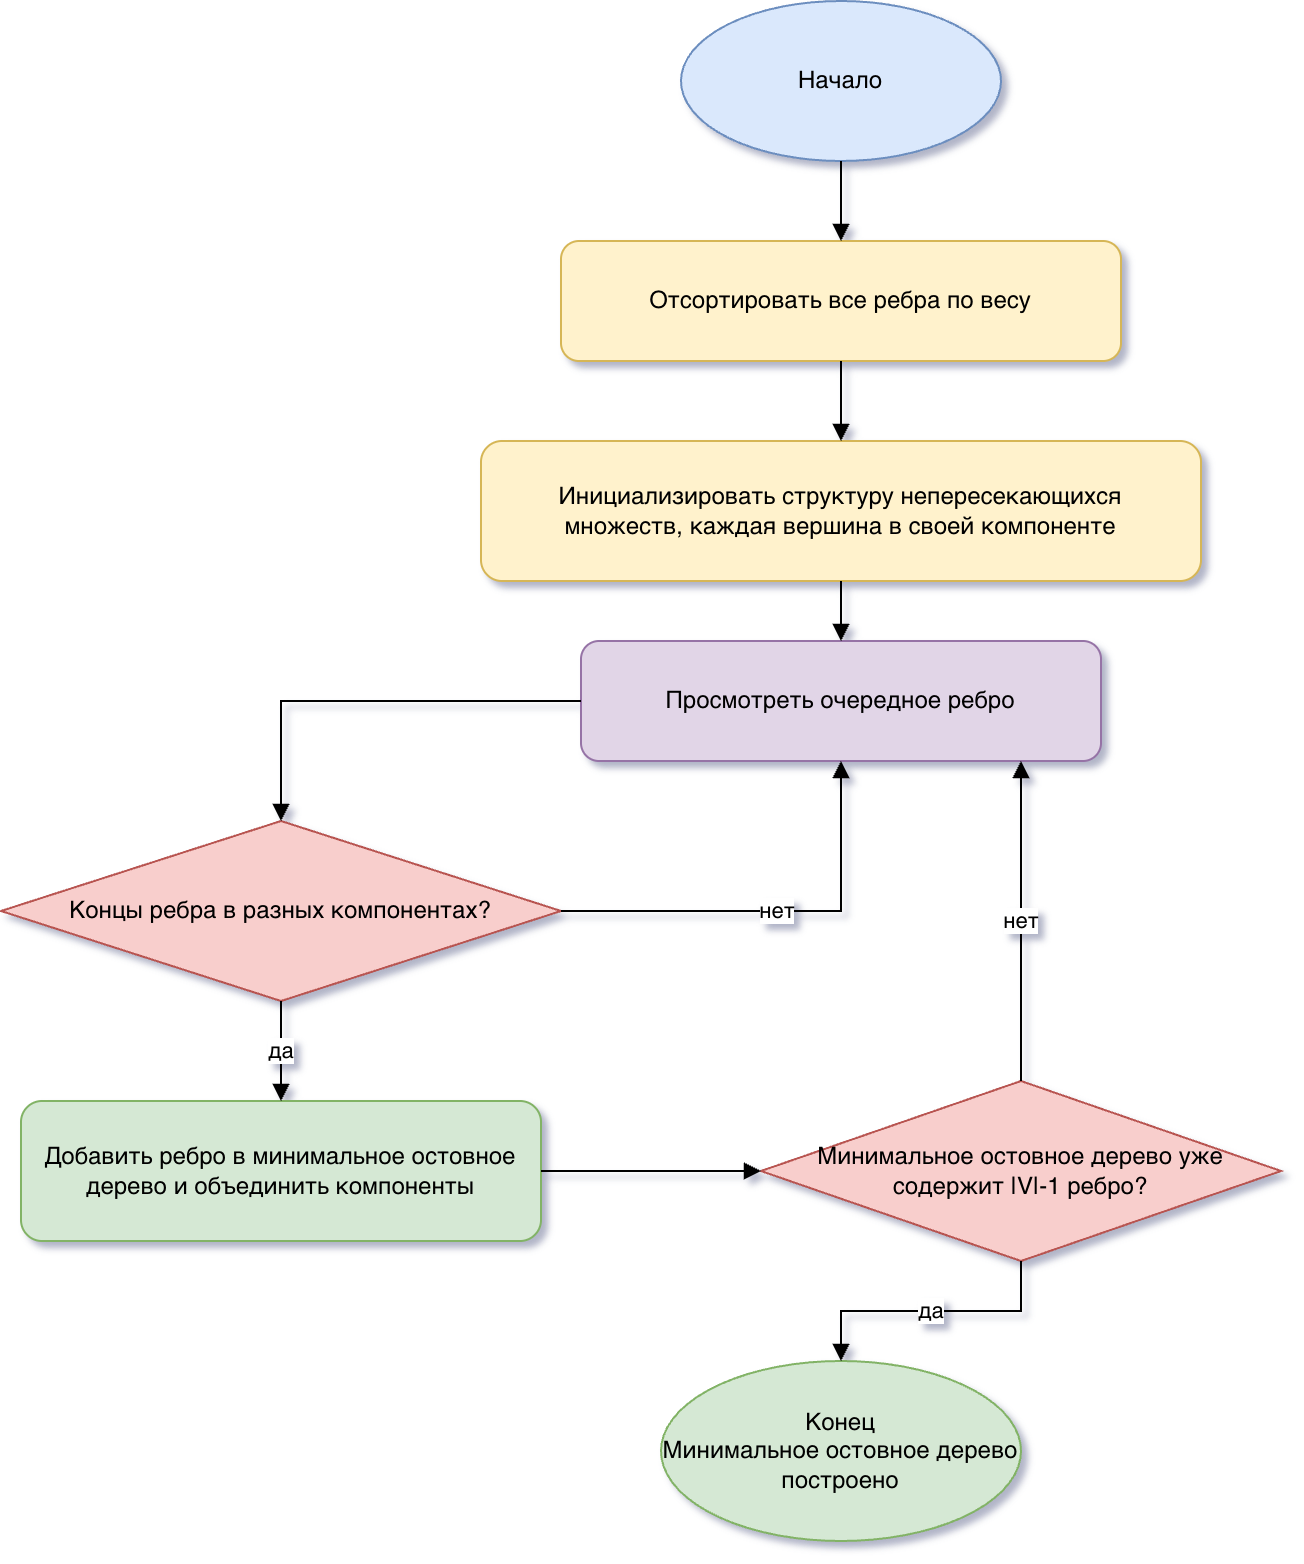
\includegraphics[width=0.9\textwidth]{data/Крускал.drawio.png}
  \caption{Блок-схема алгоритма Крускала.}
\end{figure}

\subsection{Алгоритм Прима с бинарной кучей}

Алгоритм Прима строит MST постепенно, начиная с произвольной стартовой вершины. В отличие от Крускала, он растит одно дерево, а не объединяет компоненты из набора отдельных ребер.

На каждом шаге выбирается минимальное ребро, которое соединяет уже построенную часть дерева с одной из еще не включенных вершин. Для ускорения поиска минимума используется бинарная куча.

Для каждой вершины $v$, не вошедшей в дерево, хранится минимальная известная стоимость подключения $key[v]$.
Тогда переходы между состояниями можно описать как:
\begin{equation}
  key[v] = \min_{u \in S} w(u,v),
\end{equation}
где $S$ -- множество вершин, уже вошедших в дерево.

В процессе работы алгоритма выполняются следующие действия:
\begin{enumerate}
  \item выбрать стартовую вершину;
  \item положить ее в дерево;
  \item обновить стоимости подключения для ее соседей;
  \item извлечь из кучи вершину с минимальным ключом;
  \item повторять до включения всех вершин.
\end{enumerate}

\subsection{Алгоритм Прима с кучей Фибоначчи}

Идея алгоритма остается той же, что и в предыдущем варианте. Отличие заключается в структуре очереди с приоритетом. В куче Фибоначчи операции вставки и уменьшения ключа выполняются амортизированно за $O(1)$, а извлечение минимума -- за $O(\log n)$.

Это делает структуру теоретически удобной для алгоритмов, где часто выполняется операция decrease-key. Именно поэтому куча Фибоначчи рассматривается как модификация Прима в сравнении с бинарной кучей.

\subsubsection{Блок-схема Алгоритма Прима}

\begin{figure}[H]
  \centering
  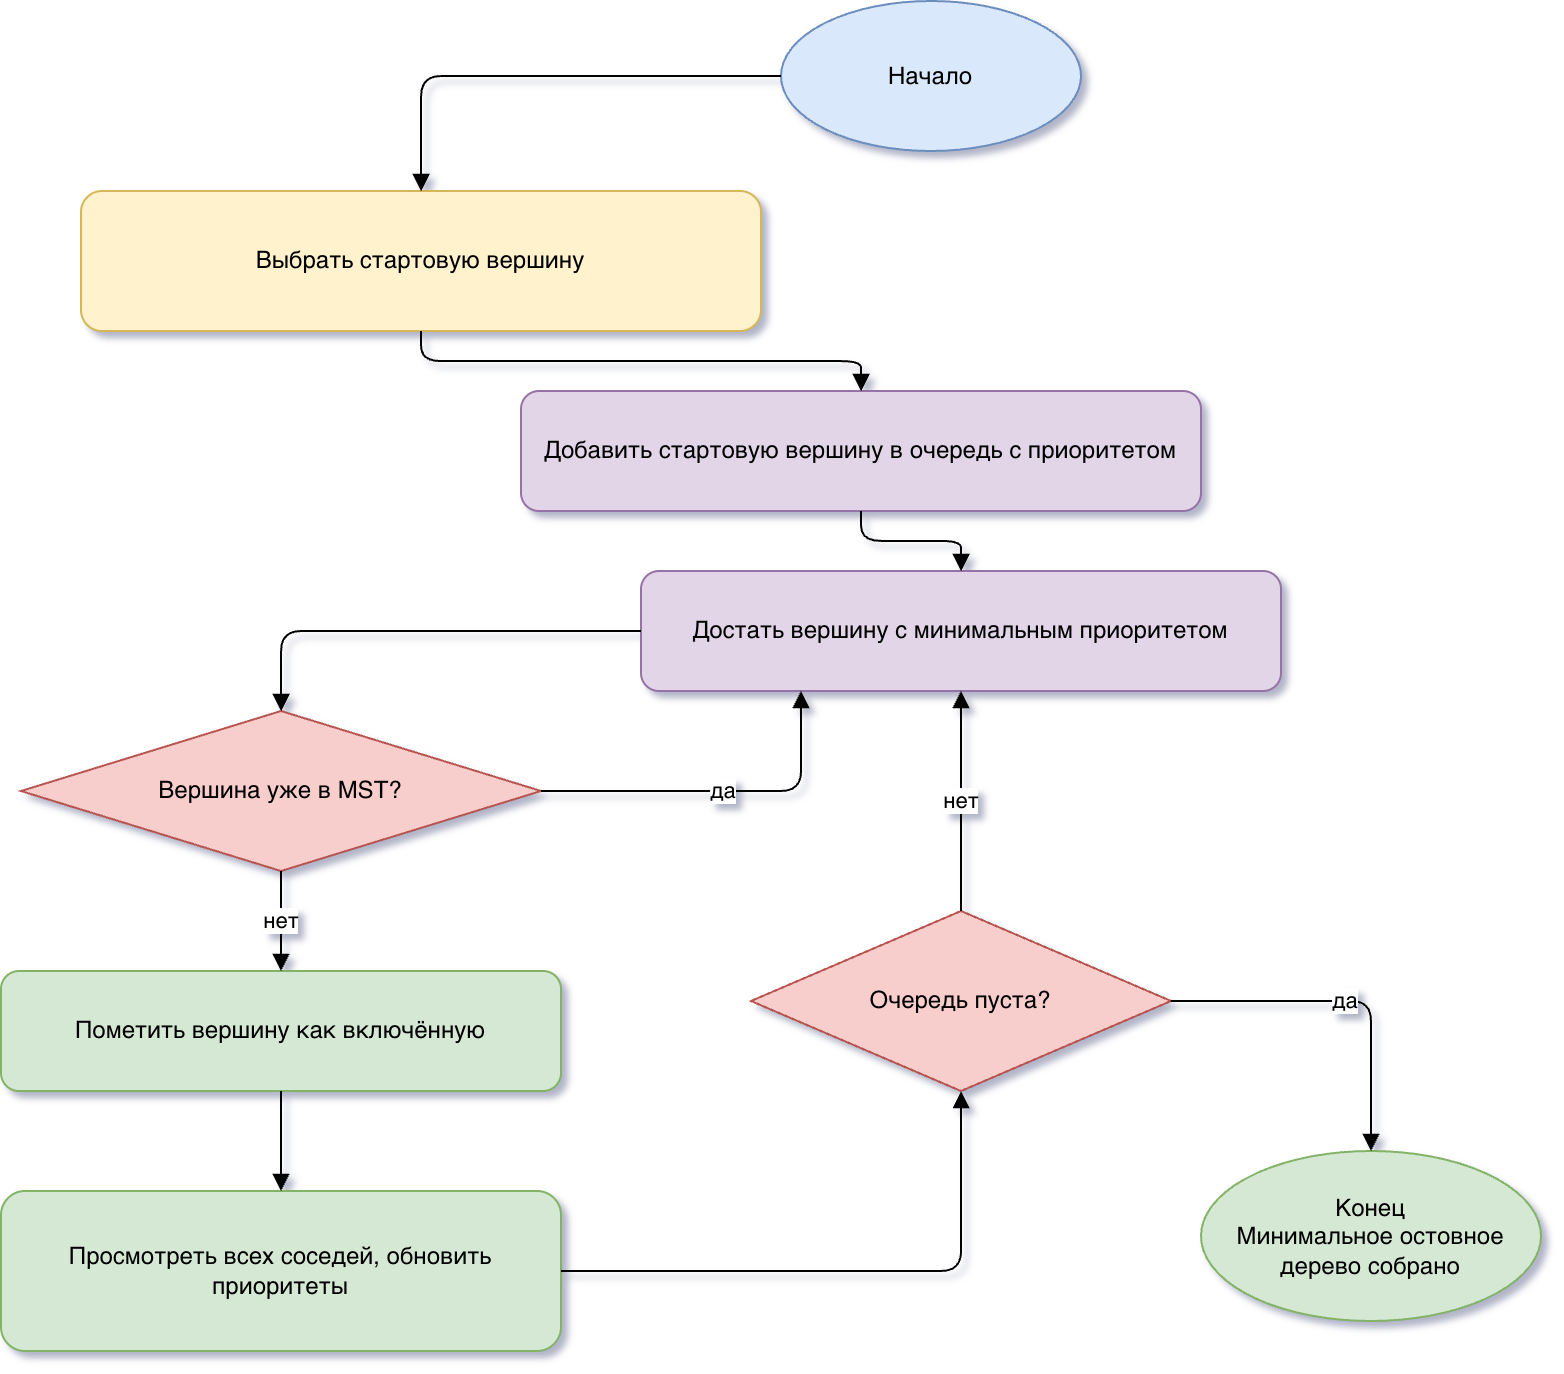
\includegraphics[width=0.9\textwidth]{data/Прим.drawio.png}
  \caption{Блок-схема алгоритма Прима.}
\end{figure}

\subsection{Алгоритм Борувки}

Алгоритм Борувки также строит MST по компонентам связности. На каждой итерации для каждой компоненты выбирается самое дешевое исходящее ребро, после чего несколько компонент могут быть объединены одновременно.

Идея метода состоит в том, что каждая компонента самостоятельно ищет ближайшего соседа. Это позволяет эффективно уменьшать число компонент на больших графах.

Пошагово алгоритм выглядит так:
\begin{enumerate}
  \item каждая вершина рассматривается как отдельная компонента;
  \item для каждой компоненты находится минимальное исходящее ребро;
  \item выбранные ребра добавляются в MST;
  \item компоненты объединяются через DSU;
  \item процесс повторяется, пока не останется одна компонента.
\end{enumerate}

\subsubsection{Блок-схема Алгоритма Борувки}

\begin{figure}[H]
  \centering
  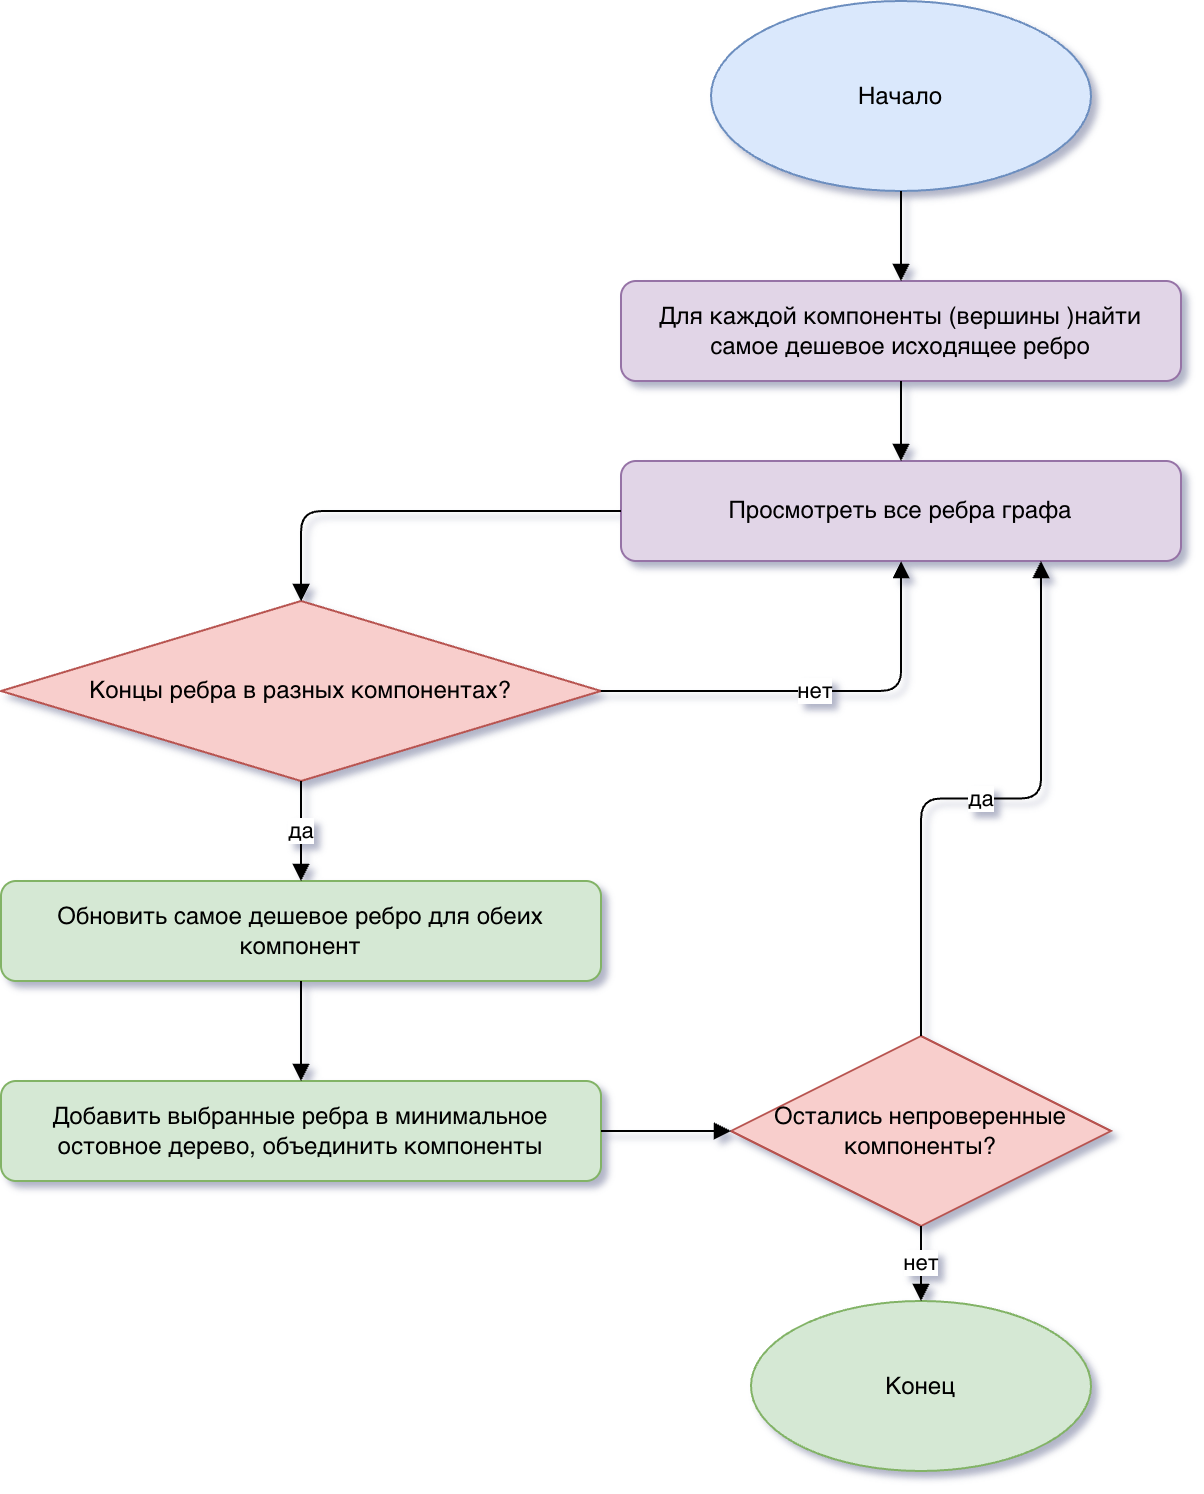
\includegraphics[width=0.9\textwidth]{data/Борувка.drawio.png}
  \caption{Блок-схема алгоритма Борувки.}
\end{figure}


\section{Формализация задачи и структура программы}
\label{sec:formalization}

Программа реализована на языке Python с использованием следующих библиотек:
\begin{enumerate}
  \item \texttt{numpy} -- генерация и обработка числовых данных;
  \item \texttt{matplotlib} -- построение графиков времени выполнения;
  \item \texttt{PyQt6} -- графический интерфейс пользователя.
\end{enumerate}

Исходный код программы имеет следующую структуру:
\begin{lstlisting}[language=bash, caption={Файловая структура проекта.}, label=lst:filetree]
main.py
benchmark.py
src/
  __init__.py
  algorithms.py
  benchmarking.py
  graph_utils.py
  ui.py
requirements.txt
\end{lstlisting}

\section{Рекомендации пользователю}
\label{sec:user_guide}

Взаимодействие с программой осуществляется через графический интерфейс. Пользователь может:
\begin{enumerate}
  \item сгенерировать граф нужной размерности;
  \item выбрать плотность графа;
  \item запустить один алгоритм или сравнение всех алгоритмов;
  \item просмотреть итоговое дерево и логи выполнения;
  \item запустить полный бенчмарк и сохранить результаты.
\end{enumerate}

\section{Рекомендации программисту}
\label{sec:dev_guide}

\textbf{Системные требования:}
\begin{itemize}
  \item операционная система Windows, Linux или macOS;
  \item свободное место на диске -- не менее 50 Мб;
  \item свободная оперативная память -- не менее 200 Мб.
\end{itemize}

\textbf{Требования к установленному ПО:}
\begin{itemize}
  \item Python 3.10+;
  \item зависимости из файла \texttt{requirements.txt}.
\end{itemize}

\textbf{Инструкция по запуску:}
\begin{enumerate}
  \item перейти в директорию проекта;
  \item создать и активировать виртуальное окружение;
  \item установить зависимости командой \texttt{pip install -r requirements.txt};
  \item запустить программу командой \texttt{python main.py}.
\end{enumerate}

Для получения таблиц и графиков бенчмарка можно дополнительно запустить:
\begin{lstlisting}[language=bash]
python benchmark.py
\end{lstlisting}

\section{Контрольный пример}
\label{sec:test_case}

Для проверки корректности была сгенерирована серия случайных связных графов. На одном и том же графе запускались все четыре алгоритма, после чего сравнивался вес найденного MST. Во всех случаях веса совпали, что подтверждает корректность реализации.

Интерфейс программы позволяет менять параметры генерации графа и повторять тестирование на разных экземплярах.

\begin{figure}[H]
  \centering
  \includegraphics[width=0.9\textwidth]{data/benchmarks/interface.png}
  \caption{Интерфейс программы.}
\end{figure}

Ниже приведены усредненные результаты тестирования для графов размерности 500, полученные в ходе полного бенчмарка.

\begin{table}[H]
  \centering
  \caption{Сводные результаты для $|V|=500$}
  \begin{tabular}{lrr}
    \toprule
    Алгоритм & Плотность & Среднее время, мс \\
    \midrule
    Крускал & 0.05 & 0.989 \\
    Прим (бинарная куча) & 0.05 & 1.525 \\
    Прим (куча Фибоначчи) & 0.05 & 3.162 \\
    Борувка & 0.05 & 5.390 \\
    Крускал & 0.20 & 3.330 \\
    Прим (бинарная куча) & 0.20 & 3.998 \\
    Прим (куча Фибоначчи) & 0.20 & 6.657 \\
    Борувка & 0.20 & 19.313 \\
    Крускал & 0.60 & 8.364 \\
    Прим (бинарная куча) & 0.60 & 13.900 \\
    Прим (куча Фибоначчи) & 0.60 & 14.073 \\
    Борувка & 0.60 & 56.477 \\
    \bottomrule
  \end{tabular}
\end{table}


\section{Исследование}
\label{sec:study_table}

Ниже приводится таблица, содержащая усреднённые времена выполнения для каждого алгоритма при разных сочетаниях числа вершин и плотности графа. Исходные данные сохранены в файле \texttt{data/benchmarks/aggregated.csv}. Комментарии к таблице пользователь добавит самостоятельно.

\begin{table}[H]
  \centering
  \caption{Усреднённые времена работы (мс) по результатам бенчмарка}
  \begin{tabularx}{\textwidth}{l *{4}{>{\raggedleft\arraybackslash}X}}
    \toprule
    Алгоритм / Параметры & $|V|=500$ & $|V|=1000$ & $|V|=1500$ & $|V|=2000$ \\
    \midrule
    \multicolumn{5}{l}{\textbf{Плотность = 0.05}} \\
    Крускал & 1.00 & 3.74 & 7.31 & 14.63 \\
    Прим (бинарная куча) & 1.63 & 5.01 & 11.73 & 32.01 \\
    Прим (Фибоначчи) & 3.18 & 7.47 & 14.30 & 38.14 \\
    Борувка & 5.19 & 21.42 & 53.02 & 107.89 \\
    \midrule
    \multicolumn{5}{l}{\textbf{Плотность = 0.20}} \\
    Крускал & 3.13 & 12.73 & 27.74 & 50.53 \\
    Прим (бинарная куча) & 4.07 & 24.01 & 66.54 & 159.42 \\
    Прим (Фибоначчи) & 5.64 & 24.02 & 66.04 & 167.34 \\
    Борувка & 18.83 & 94.64 & 198.38 & 427.09 \\
    \midrule
    \multicolumn{5}{l}{\textbf{Плотность = 0.60}} \\
    Крускал & 8.37 & 35.87 & 82.18 & 145.35 \\
    Прим (бинарная куча) & 14.13 & 106.92 & 341.25 & 505.60 \\
    Прим (Фибоначчи) & 14.69 & 106.76 & 269.95 & 502.63 \\
    Борувка & 57.24 & 304.86 & 617.57 & 1245.29 \\
    \midrule
    \multicolumn{5}{l}{\textbf{Плотность = 0.85}} \\
    Крускал & 12.14 & 51.04 & 115.71 & 206.51 \\
    Прим (бинарная куча) & 21.62 & 147.09 & 390.45 & 709.70 \\
    Прим (Фибоначчи) & 19.81 & 148.44 & 394.32 & 687.92 \\
    Борувка & 79.39 & 395.86 & 989.40 & 1704.85 \\
    \bottomrule
  \end{tabularx}
\end{table}

\begin{figure}[H]
  \centering
  \includegraphics[width=0.9\textwidth]{data/benchmarks/runtime_0_05.png}
  \caption{Зависимость времени работы от числа вершин для плотности 0.05.}
\end{figure}

На графах с низкой плотностью (0.05) алгоритмы Прима с обоими типами куч показывают близкую производительность, а алгоритм Крускала работает быстрее. Алгоритм Борувки значительно отстает по времени.

\begin{figure}[H]
  \centering
  \includegraphics[width=0.9\textwidth]{data/benchmarks/runtime_0_20.png}
  \caption{Зависимость времени работы от числа вершин для плотности 0.20.}
\end{figure}

При увеличении плотности до 0.20 алгоритмы Прима начинают отставать от Крускала, а Борувка становится еще менее эффективным. Разница между бинарной и Фибоначчи кучами становится менее заметной.

\begin{figure}[H]
  \centering
  \includegraphics[width=0.9\textwidth]{data/benchmarks/runtime_0_60.png}
  \caption{Зависимость времени работы от числа вершин для плотности 0.60.}
\end{figure}

На плотных графах (0.60) ситуация практически не меняется: Крускал остается самым быстрым, алгоритмы Прима значительно отстают, а Борувка становится крайне неэффективной.

\begin{figure}[H]
  \centering
  \includegraphics[width=0.9\textwidth]{data/benchmarks/runtime_0_85.png}
  \caption{Зависимость времени работы от числа вершин для плотности 0.85.}
\end{figure}

При плотности 0.85 все алгоритмы заметно замедляются, но Крускал сохраняет преимущество. Алгоритмы Прима с обоими типами куч показывают схожую производительность, а Борувка становится практически непригодной для больших графов.

\section{Выводы}
\label{sec:analysis}

По результатам экспериментов можно сделать следующие выводы:
\begin{enumerate}
  \item В подавляющем большинстве случаев алгоритм Крускала показывает лучшую производительность, особенно на разреженных графах.
  \item Алгоритмы Прима с бинарной и Фибоначчи кучами демонстрируют схожую производительность, что может быть связано с тем, что в нашем тестовом наборе не было достаточно больших графов, где преимущества Фибоначчи кучи могли бы проявиться.
  \item Алгоритм Борувки значительно отстает от остальных, особенно на плотных графах, что делает его неэффективным для практического использования в таких случаях.
  \item С увеличением плотности графа все алгоритмы замедляются, но Крускал сохраняет преимущество, что подтверждает его эффективность для широкого диапазона графов.
\end{enumerate}

Таким образом, наиболее универсальным и эффективным алгоритмом для построения минимального остовного дерева в нашем тестовом наборе является алгоритм Крускала. Алгоритмы Прима с различными типами куч могут быть полезны в специфических случаях, но в целом не показывают значительного преимущества. Алгоритм Борувки, несмотря на свою теоретическую привлекательность, оказывается неэффективным на практике для графов с высокой плотностью.


\end{document}
